\documentclass[9pt, aspectratio=169]{beamer}

\usetheme{metropolis}
\setbeamertemplate{itemize items}{\faAngleRight}

\metroset{titleformat=smallcaps,block=fill,numbering=counter,progressbar=frametitle,sectionpage=none}
\setbeamersize{text margin left=5mm,text margin right=5mm} 
% %%%%%%%%%%%%%%%%%%%%%%%%%%%%%%%%%%%%%%%%%%%%%%%%%%%%%%%%%%%%%%%%%%%%%%%%%%%%%%
% \embedvideo{<poster or text>}{<video file (MP4+H264)>}
% \embedvideo*{...}{...}                     % auto-play
%%%%%%%%%%%%%%%%%%%%%%%%%%%%%%%%%%%%%%%%%%%%%%%%%%%%%%%%%%%%%%%%%%%%%%%%%%%%%%

\usepackage[bigfiles]{pdfbase}
\ExplSyntaxOn
\NewDocumentCommand\embedvideo{smm}{
  \group_begin:
  \leavevmode
  \tl_if_exist:cTF{file_\file_mdfive_hash:n{#3}}{
    \tl_set_eq:Nc\video{file_\file_mdfive_hash:n{#3}}
  }{
    \IfFileExists{#3}{}{\GenericError{}{File~`#3'~not~found}{}{}}
    \pbs_pdfobj:nnn{}{fstream}{{}{#3}}
    \pbs_pdfobj:nnn{}{dict}{
      /Type/Filespec/F~(#3)/UF~(#3)
      /EF~<</F~\pbs_pdflastobj:>>
    }
    \tl_set:Nx\video{\pbs_pdflastobj:}
    \tl_gset_eq:cN{file_\file_mdfive_hash:n{#3}}\video
  }
  %
  \pbs_pdfobj:nnn{}{dict}{
    /Type/RichMediaInstance/Subtype/Video
    /Asset~\video
    /Params~<</FlashVars (
      source=#3&
      skin=SkinOverAllNoFullNoCaption.swf&
      skinAutoHide=true&
      skinBackgroundColor=0x5F5F5F&
      skinBackgroundAlpha=0
    )>>
  }
  %
  \pbs_pdfobj:nnn{}{dict}{
    /Type/RichMediaConfiguration/Subtype/Video
    /Instances~[\pbs_pdflastobj:]
  }
  %
  \pbs_pdfobj:nnn{}{dict}{
    /Type/RichMediaContent
    /Assets~<<
      /Names~[(#3)~\video]
    >>
    /Configurations~[\pbs_pdflastobj:]
  }
  \tl_set:Nx\rmcontent{\pbs_pdflastobj:}
  %
  \pbs_pdfobj:nnn{}{dict}{
    /Activation~<<
      /Condition/\IfBooleanTF{#1}{PV}{XA}
      /Presentation~<</Style/Embedded>>
    >>
    /Deactivation~<</Condition/PI>>
  }
  %
  \hbox_set:Nn\l_tmpa_box{#2}
  \tl_set:Nx\l_box_wd_tl{\dim_use:N\box_wd:N\l_tmpa_box}
  \tl_set:Nx\l_box_ht_tl{\dim_use:N\box_ht:N\l_tmpa_box}
  \tl_set:Nx\l_box_dp_tl{\dim_use:N\box_dp:N\l_tmpa_box}
  \pbs_pdfxform:nnnnn{1}{1}{}{}{\l_tmpa_box}
  %
  \pbs_pdfannot:nnnn{\l_box_wd_tl}{\l_box_ht_tl}{\l_box_dp_tl}{
    /Subtype/RichMedia
    /BS~<</W~0/S/S>>
    /Contents~(embedded~video~file:#3)
    /NM~(rma:#3)
    /AP~<</N~\pbs_pdflastxform:>>
    /RichMediaSettings~\pbs_pdflastobj:
    /RichMediaContent~\rmcontent
  }
  \phantom{#2}
  \group_end:
}
\ExplSyntaxOff
%%%%%%%%%%%%%%%%%%%%%%%%%%%%%%%%%%%%%%%%%%%%%%%%%%%%%%%%%%%%%%%%%%%%%%%%%%%%%%

\usepackage{fontspec,minted}
\usepackage[scale=1]{ccicons}
\usepackage{metalogo}
\usepackage{xcolor,colortbl}
\usepackage{multicol,multirow,booktabs}
\usepackage{appendixnumberbeamer}
\usepackage{graphicx}
\usepackage{bm}
\usepackage{fontawesome}
\usepackage{csquotes}
\usepackage[backend=biber, natbib, sorting=nyt, doi=true, url=false, url=false, isbn=false, maxbibnames=10]{biblatex}
\addbibresource{../../utils/refs.bib}

\usepackage[spanish]{babel}
\usepackage{mathtools}
\usefonttheme{professionalfonts}
\usepackage{textcomp}

\setsansfont[BoldFont={Iwona Bold}, Numbers={Lining, Proportional}]{Iwona Light}
% \setmathsfont(Digits)[Numbers={Lining, Proportional}]{Fira Sans Light}
\setmonofont[Scale=MatchLowercase]{DejaVu Sans Mono}

\setbeamercolor{alerted text}{fg=red,bg=black!2}
\setbeamercolor{progress bar}{fg=red,bg=red!2}
\setbeamertemplate{itemize item}{\faCaretRight}
\setbeamertemplate{itemize subitem}{ \faAngleRight}
\setbeamertemplate{blocks}[shadow=false]
\setbeamercolor{block title}{bg=black!30,fg=red}
\setbeamercolor{block body}{bg=black!20,fg=black}
 
\usepackage{gensymb,amssymb}
\usepackage{upquote}
\usepackage{algpseudocode}
\algrenewcommand\algorithmicrequire{\textbf{Requiere}}
\algrenewcommand\algorithmicensure{\textbf{Devuelve}}
%\setbeamertemplate{blocks}[rounded][shadow=false]
\setbeamertemplate{blocks}[shadow=false]

\newcommand{\cx}{\column{0.5\textwidth}}
\newcommand{\cw}[1]{\column{#1\textwidth}}

\author{Manuel Carlevaro}
\date{{\tiny Departamento de Ingeniería Mecánica \\[-1em]
             Grupo de Materiales Granulares - UTN FRLP \\
        \faEnvelope{} manuel.carlevaro@gmail.com \- $\cdot$ \- \faTwitter{} @mcarlevaro}}
\institute{
  \vspace{6em}
  \centering
  {\tiny
  Cálculo Avanzado \enspace • \enspace 2022 \\
    \faLinux \- $\cdot$ \- \fontspec{TeX Gyre Pagella}\XeLaTeX \- $\cdot$ \- \ccbysa }
}

%% Operadores
\DeclareMathOperator{\sen}{sen}
\DeclareMathOperator{\sign}{sign}
\newcommand{\T}[1]{\underline{\bm{#1}}}
\DeclareMathOperator{\Tr}{Tr}

\usepackage{hyperref}
\hypersetup{
    colorlinks,
    citecolor=blue,
    filecolor=black,
    linkcolor=blue,
    urlcolor=blue
}
\urlstyle{same}

%% Códigos
\usepackage{minted}
\newminted[cpp]{cpp}{linenos,fontsize=\footnotesize,frame=lines,numbersep=4pt}
\newmintedfile[cppcode]{cpp}{linenos,fontsize=\footnotesize,frame=lines,numbersep=4pt}
\newcommand{\mic}[1]{\mintinline{C++}{#1}}

\newminted[py]{python}{linenos,fontsize=\footnotesize,frame=lines,numbersep=4pt}
\newminted[pyc]{pycon}{linenos,fontsize=\footnotesize,frame=lines,numbersep=4pt} % Consola de Python
\newminted[ipy3]{ipython3}{linenos,fontsize=\footnotesize,frame=lines,numbersep=4pt} % Consola de iPython3
\newmintedfile[pycode]{python}{linenos,fontsize=\footnotesize,frame=lines,numbersep=4pt}

\newmintedfile[makef]{basemake}{linenos,fontsize=\footnotesize,frame=lines,numbersep=4pt}
\definecolor{bg}{RGB}{22,43,58}
\newminted[shell]{console}{linenos=false,fontsize=\footnotesize,breaklines=true, frame=single} % Linea de comandos
\renewcommand\listingscaption{Código}

\makeatletter
\AtBeginEnvironment{minted}{\dontdofcolorbox}
\def\dontdofcolorbox{\renewcommand\fcolorbox[4][]{##4}}
\makeatother

% uso:
% Ejemplo de uso explícito:
% \begin{py}
% >>> list("abcd")
% ['a', 'b', 'c', 'd']
% \end{py}
% 
% Ahora ejemplo de código en file:
% \pycode{Chapters/intro/code/hola.py}
% 
% También se puede poner un sector del file:
% \pycode[firstline=6, lastline=7]{Chapters/intro/code/hola.py}
% 
% También se puede poner código \textit{inline}: \mip{print('¡Hola mundo!')} y en una sola línea:
% \slp|if __name__ == '__main__')|
% 
% Por último, se puede poner el código en un entorno \textit{float}, esto es, como las tablas y las figuras, con un caption y un label para luego hacer referencias, como por ejemplo al Código \ref{code:hola}.


\usepackage{tikz}
\usetikzlibrary{shapes,shadows,arrows,positioning,matrix,chains,backgrounds,fit}

\tikzset{
    %Define standard arrow tip
    >=stealth',
    %Define style for boxes
    obj/.style={
           rectangle,
           rounded corners,
           draw, very thick,
           text width=10em, fill=green!20,
           minimum height=2em,
           text centered, drop shadow},
    proc/.style={
	    rectangle, rounded corners,
	    draw,fill=red!50,very thick,
	    text width=8em,minimum height=2em,
	    text centered, drop shadow},
    % Define arrow style
    pil/.style={
           ->,
           thick,
           shorten <=2pt,
           shorten >=2pt,}
}

\setbeamertemplate{bibliography item}{%
  \ifboolexpr{ test {\ifentrytype{book}} or test {\ifentrytype{mvbook}}
    or test {\ifentrytype{collection}} or test {\ifentrytype{mvcollection}}
    or test {\ifentrytype{reference}} or test {\ifentrytype{mvreference}} }
    {\setbeamertemplate{bibliography item}{\faBook}}
    {\ifentrytype{online}
            {\setbeamertemplate{bibliography item}{\faGlobe}}
   {\setbeamertemplate{bibliography item}{\faFileText}}}%
  \usebeamertemplate{bibliography item}}

\defbibenvironment{bibliography}
  {\list{}
     {\settowidth{\labelwidth}{\usebeamertemplate{bibliography item}}%
      \setlength{\leftmargin}{\labelwidth}%
      \setlength{\labelsep}{\biblabelsep}%
      \addtolength{\leftmargin}{\labelsep}%
      \setlength{\itemsep}{\bibitemsep}%
      \setlength{\parsep}{\bibparsep}}}
  {\endlist}
  {\item}
\newcommand{\bcite}[1]{\citeauthor{#1}, \citetitle{#1} (\citeyear{#1})}


\title{Autovalores y autovectores}
\subtitle{Definiciones. Interpretación geométrica. Círculos de Gerschgorin. Método de las potencias. Método de la potencia: código. Factorización QR. Código.}

%%%%
% Bibliografía
%%%%

\begin{document}
\maketitle

\begin{frame}
\begin{columns}[t]
\cx
\begin{definition}[Autovalor y autovector]
    Sea $\bm{A} \in K^{n \times n}$ y $\bm{v} \in K^n$. $\bm{v}$ es un \textbf{autovector} de $\bm{A}$ si 
    \[ \bm{A} \bm{v} = \lambda \bm{v} \]
    donde $\lambda$ es un escalar en $K$, denominado \textbf{autovalor} asociado con $\bm{v}$.
\end{definition}  \pause
En forma equivalente:
\begin{equation}
(\bm{A} - \lambda \bm{I}) \bm{v} = \bm{0}
\label{eq:avv01}
\end{equation}
Este sistema tiene solución $\bm{v} \neq \bm{0}$ si y solo si:
\[ \det(\bm{A} - \lambda \bm{I}) = 0 \]
denominado \textbf{polinomio característico}, $p_A(\lambda)$, y por el teorema fundamental del álgebra: $\mapsto n$ raíces.
\pause  

\cx
\textbf{Ejemplo:}
\[ \bm{A} = \begin{bmatrix}
    3 & -1 & 0 \\
    -1 & 2 & -1 \\
    0 & -1 & 3
\end{bmatrix} \]
\begin{align*}
   p_A(\lambda) =  \det(\bm{A} - \lambda \bm{I}) &= 
    \begin{vmatrix}
        3 - \lambda & -1 & 0 \\
        -1 & 2 - \lambda & -1 \\
        0 & -1 & 3 - \lambda
    \end{vmatrix} \\
   &= -\lambda^3 +8 \lambda^2 - 19 \lambda + 12 = 0
\end{align*}
Solución: $\lambda_1 = 1, \lambda_2 = 3, \lambda_3 = 4$. Reemplazando cada autovalor en \eqref{eq:avv01}:
\[ \bm{v}_1 = a \begin{bmatrix} 1 \\ 2 \\ 1 \end{bmatrix}, 
 \bm{v}_2 = b \begin{bmatrix} 1 \\ 0 \\ -1 \end{bmatrix}, 
 \bm{v}_3 = c \begin{bmatrix} 1 \\ -1 \\ 1 \end{bmatrix} \]
 \pause
\textbf{Definiciones:}
\begin{equation*}
    \begin{split}
        \text{Espectro de } \bm{A}&: \sigma(\bm{A}) = \{\lambda_1, \lambda_2, \cdots, \lambda_n \} \\
    \text{Radio espectral de } \bm{A}&: \rho(\bm{A}) = \max_{\lambda \in \sigma(\bm{A})}|\lambda|
    \end{split}
\end{equation*}
\end{columns}
\end{frame}

\begin{frame}
\begin{columns}[t]
\cw{0.3}
\textbf{Intepretación gráfica}
\begin{center}
    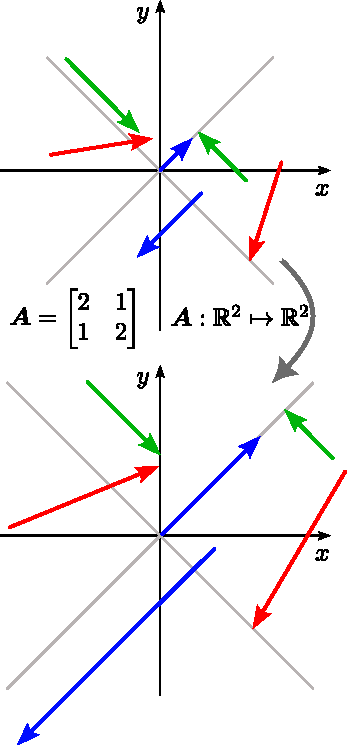
\includegraphics[height=1.0\textheight]{figs/autovalvec-01.pdf}
\end{center}

\cw{0.6}
\begin{align*}
    p_A(\lambda) &= \det(\bm{A} - \lambda \bm{I}) = \begin{vmatrix} 2 - \lambda & 1 \\ 1 & 2 - \lambda \end{vmatrix} \\
                 &= (2 - \lambda)^2 - 1 = \lambda^2 - 4 \lambda + 3 = (\lambda - 3)(\lambda - 1) = 0
\end{align*} \pause

Con $\lambda_1 = 3$:
\[ \begin{cases}
    (2 - 3) x + y &= 0 \\
    x + (2 - 3) y &= 0
\end{cases} \Longrightarrow \bm{v}_1 = \begin{bmatrix} 1 \\ 1 \end{bmatrix} 
\] \pause
Con $\lambda_2 = 1$:
\[ \begin{cases}
    (2 - 1) x + y &= 0 \\
    x + (2 - 1) y &= 0
\end{cases} \Longrightarrow \bm{v}_2 = \begin{bmatrix} 1 \\ -1 \end{bmatrix} 
\]
\hrulefill

\textbf{Nota:} si consideramos la norma vectorial $l_2: \lVert \cdot \rVert$:
\[ \lVert \bm{A} \rVert_2 = \rho(\bm{A}^{\dag} \bm{A})^{1/2} \]
Si $\bm{A}$ es simétrica, $\lVert \bm{A} \rVert_2 = \rho(\bm{A})$.
\end{columns}
\end{frame}

\begin{frame}
\begin{columns}[t]
\cx
\textbf{Métodos:}
\begin{itemize}
    \item Analítico: $n < 5$.
    \item Parciales: computan solo autovalores \textbf{extremos} (módulo máximo o mínimo). Método de las potencias.
    \item Globales: aproximan a todo el \textbf{espectro} de $\bm{A}$, $\sigma(\bm{A})$. Método $QR$.
\end{itemize}
\hrulefill \pause

\begin{theorem}[Círculo de Gerschgorin]
    $\bm{A} \in K^{n \times n}$, $r_i = \sum_{j \neq i}^n |a_{ij}|$ para cada $i = 1, 2, \cdots, n$. Sea
    \[ C_i = \{ z \in \mathbb{C} : |z - a_{ii}| \leq r_i \} \]
    \vspace{-2em}
    \begin{enumerate}
        \item Si $\lambda$ es un autovalor, está en uno de los $C_i$.
        \item Si $k$ círculos $C_i$ forman una región conectada $R \in \mathbb{C}$, dijunta de los restantes $n - k$ círculos, entonces $R$ contiene exactamente $k$ autovalores.
    \end{enumerate}
\end{theorem} \pause

\cx
\textbf{Ejemplo:}
\[ \begin{bmatrix}
    1 & - 1 & 0 \\
    1 & 5 & 1 \\
    -2 & -1 & 9
\end{bmatrix} \]
{\small $r_1 = |-1| + |0| = 1, r_2 = |1| + |1| = 2, r_3 = |-2| + |-1| = 3$.}
{\small $\lambda_1 = 1.33192769, \lambda_2 = 8.81113862, \lambda_3 = 4.85693369$ }.
\begin{center}
    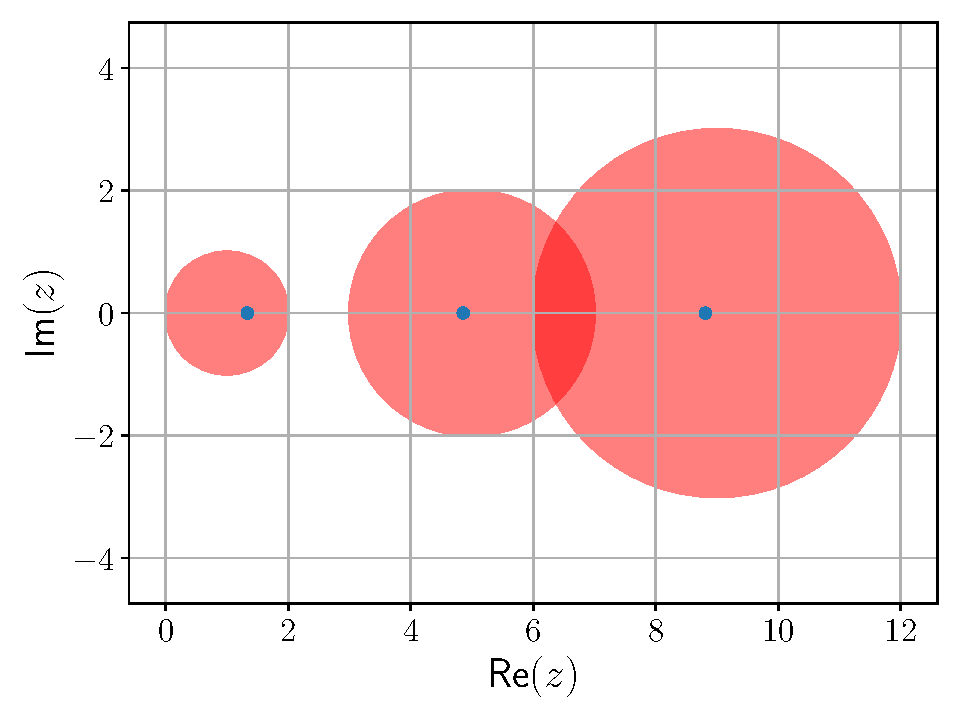
\includegraphics[width=1.0\textwidth]{figs/circles.pdf}
\end{center}
\end{columns}
\end{frame}


\begin{frame}
\begin{columns}[t]
\cx
\textbf{Método de las potencias:}

$\bm{A} \in \mathbb{R}^{n \times n}$, con elementos de $\sigma(\bm{A})$ que satisfacen:$|\lambda_1| > |\lambda_2| \geq |\lambda_3| \geq \cdots \geq |\lambda_n|$. $\lambda_1$: \textbf{autovalor dominante}. $\{ \bm{v}_1, \bm{v}_2, \cdots,\bm{v}_n \}$ forman una \textbf{base} en $\mathbb{R}^n$ (linealmente independientes).
\[ \bm{x} = \sum_{j=1}^n \beta_j \bm{v}_j \]
Multiplicando ambos miembros por $\bm{A}, \bm{A}^2, \cdots, \bm{A}^k, \cdots$:
\begin{align*}
    \bm{A} \bm{x} &= \sum_{j=1}^n \beta_j \bm{A} \bm{v}_j = \sum_{j=1}^n \beta_j \lambda_j \bm{v}_j \\ 
    \bm{A}^2 \bm{x} &= \sum_{j=1}^n \beta_j \lambda_j \bm{A} \bm{v}_j = \sum_{j=1}^n \beta_j \lambda_j^2 \bm{v}_j \\ 
                    &\vdots \\
    \bm{A}^k \bm{x} &= \sum_{j=1}^n \beta_j \lambda_j^k \bm{v}_j \\ 
\end{align*}
 
\cx
Factorizando $\lambda_1$ en la última ecuación:
\[ \bm{A}^k \bm{x} = \lambda_1^k \sum_{j=1}^n \beta_j \left(\frac{\lambda_j}{\lambda_1}\right)^k \bm{v}_j \]
Dado que $\forall j, \,|\lambda_1| > |\lambda_j|; \lim_{k \rightarrow \infty} (\lambda_j/\lambda_1)^k = 0$, y
\begin{equation} \lim_{k \rightarrow \infty} \bm{A}^k \bm{x} = \lim_{k \rightarrow \infty} \lambda_1^k \beta_1 \bm{v}_1 \label{eq:avv02} \end{equation}
Si $|\lambda_1| < 1$, \eqref{eq:avv02} $\mapsto \bm{0}$, si $|\lambda_1| > 1$, \eqref{eq:avv02} diverge ($\beta_1 \neq 0$). Elegimos $\bm{x} = \bm{x}^{(0)}$ con $\lVert \cdot \rVert_{\infty}$: $x_{p_0}^{(0)}$ con 
\[ x_{p_0}^{(0)} = 1 = \lVert \bm{x}^{(0)} \rVert_{\infty} \]
Hacemos $\bm{y}_{(1)} = \bm{A} \bm{x}^{(0)}$ y definimos $\mu^{(1)} = y_{p_0}^{(1)}$:
\begin{align*}
    \mu^{(1)} &= y_{p_0}^{(1)} = \frac{y_{p_1}^{(1)}}{x_{p_0}^{(0)}} = \frac{\beta_1 \lambda_1 v_{p_0}^{(1)} + \sum_{j=2}^n \beta_j \lambda_j v_{p_0}^{(j)}}{\beta_1 v_{p_0}^{(1)} + \sum_{j=2}^n \beta_j v_{p_0}^{(j)}} \\
              &= \lambda_1 \left[ \frac{\beta_1 v_{p_0}^{(1)} + \sum_{j=2}^n \beta_j (\lambda_j/\lambda_1) v_{p_0}^{(j)}}{\beta_1 v_{p_0}^{(1)} + \sum_{j=2}^n \beta_j v_{p_0}^{(j)}} \right]
\end{align*}
\end{columns}
\end{frame}

\begin{frame}
\vspace{1em}
\begin{columns}[t]
\cx
Sea $p_1$ el menor entero tal que $|y_{p_1}^{(1)}| = \lVert \bm{y}^{(1)} \rVert_{\infty}$:
\[ \bm{x}^{(1)} = \frac{\bm{y}^{(1)}}{y_{p_1}^{(1)}} = \frac{1}{y_{p_1}^{(1)}} \bm{A} \bm{x}^{(0)} \]
Entonces: $x_{p_1}^{(1)} = 1 = \lVert \bm{x}^{(1)} \rVert_{\infty}$. Ahora
\[ \bm{y}^{(2)} = \bm{A} \bm{x}^{(1)} = \frac{1}{y_{p_1}^{(1)}} \bm{A}^2 \bm{x}^{(0)} \]
y
\begin{align*}
    \mu^{(2)} &= y_{p_1}^{(2)} = \frac{y_{p_1}^{(2)}}{x_{p_1}^{(1)}} = \frac{ \left[ \beta_1 \lambda_1^2 v_{p_1}^{(1)} + \sum_{j=2}^n \beta_j \lambda_j^2 v_{p_1}^{(j)} \middle/ y_{p_1}^{(1)} \right]}{ \left[ \beta_1 \lambda_1 v_{p_1}^{(1)} + \sum_{j=2}^n \beta_j \lambda_j v_{p_1}^{(j)} \middle/ y_{p_1}^{(1)} \right]} \\
              &= \lambda_1 \left[ \frac{\beta_1 v_{p_1}^{(1)} + \sum_{j=2}^n \beta_j (\lambda_j/\lambda_1)^2 v_{p_1}^{(j)}}{\beta_1 v_{p_1}^{(1)} + \sum_{j=2}^n \beta_j (\lambda_j/\lambda_1) v_{p_1}^{(j)}} \right]
\end{align*}
Sea $p_2$ el menor entero tal que $|y_{p_2}^{(2)}| = \lVert \bm{y}^{(2)} \rVert_{\infty}$:
\[ \bm{x}^{(2)} = \frac{\bm{y}^{(2)}}{y_{p_2}^{(2)}} = \frac{1}{y_{p_2}^{(2)}} \bm{A} \bm{x}^{(1)} = \frac{1}{y_{p_2}^{(2)} y_{p_1}^{(1)}} \bm{A}^2 \bm{x}^{(0)} \]

\cx
$\mapsto$ secuencias $\{ \bm{x}^{(m)} \}_{m=0}^{\infty}$, $\{ \bm{y}^{(m)} \}_{m=0}^{\infty}$, $\{ \mu^{(m)} \}_{m=0}^{\infty}$, inductivamente:
\[ \bm{y}^{(m)} = \bm{A} \bm{x}^{(m-1)} \] 
\begin{align*} \mu^{(m)} &= y_{p_{m - 1}}^{(m)} \\
&= \lambda_1 \left[ \frac{\beta_1 v_{p_{m-1}}^{(1)} + \sum_{j=2}^n (\lambda_j/\lambda_1)^m \beta_j v_{p_{m-1}}^{(j)}}{\beta_1 v_{p_{m-1}}^{(1)} + \sum_{j=2}^n (\lambda_j/\lambda_1)^{m-1} \beta_j v_{p_{m-1}}^{(j)}} \right] \end{align*}
y
\[ \bm{x}^{(m)} = \frac{\bm{y}^{(m)}}{y_{p_{m}^{(m)}}} = \frac{\bm{A}^m \bm{x}^{(0)}}{ \prod_{k=1}^m y_{p_k}^{(k)}} \]
donde para cada paso, $p_m$ es el menor entero para el cual $|y_{p_m}^{(m)}| = \lVert \bm{y}^{(m)} \rVert_{\infty}$.

Dado que $|\lambda_j/\lambda_1| < 1, j=2, \cdots, n$, $\lim_{m \rightarrow \infty} \mu^{(m)} = \lambda_1$, eligiendo $\bm{x}^{(0)}$ tal que $\beta_1 \neq 0$. Además, la secuencia $\{ \bm{x}^{(m)} \}_{m=0}^{\infty}$ converge al autovalor asociado con $\lambda_1$ con norma $l_{\infty}$ igual a 1.
\end{columns}
\end{frame}

\begin{frame}
\begin{columns}[t]
\cx
\textbf{Ejemplo:}
\[ \bm{A} = \begin{bmatrix} -2 & -3 \\ 6 & 7 \end{bmatrix}, \bm{v}_1 = \begin{bmatrix} 1 \\ -2 \end{bmatrix}, \bm{v}_2 = \begin{bmatrix} 1 \\ -1 \end{bmatrix}  \]
Con $\sigma(\bm{A}) = \{4, 1\}$. Tomemos $\bm{x}^{(0)} = [1, 1]^{\intercal}$:
\begin{align*} 
    \bm{x}^{(1)} &= \bm{A} \bm{x}^{(0)} = \begin{bmatrix} -5 \\ 13 \end{bmatrix},  \bm{x}^{(2)} = \bm{A} \bm{x}^{(1)} = \begin{bmatrix} -29 \\ 61 \end{bmatrix} \\
    \bm{x}^{(3)} &= \bm{A} \bm{x}^{(2)} = \begin{bmatrix} -125 \\ 253 \end{bmatrix},  \bm{x}^{(4)} = \bm{A} \bm{x}^{(3)} = \begin{bmatrix} -509 \\ 1021 \end{bmatrix} \\
    \bm{x}^{(5)} &= \bm{A} \bm{x}^{(4)} = \begin{bmatrix} -2045 \\ 4093 \end{bmatrix},  \bm{x}^{(6)} = \bm{A} \bm{x}^{(5)} = \begin{bmatrix} -8189 \\ 16381 \end{bmatrix} 
\end{align*}

\cx
Aproximaciones al autovalor dominante $\lambda_1$:
\begin{align*}
    \lambda_1^{(1)} &= \frac{61}{13} = 4.6923, &\lambda_1^{(2)} = \frac{253}{61} = 4.14654 \\
    \lambda_1^{(3)} &= \frac{1021}{253} = 4.03557, &\lambda_1^{(4)} = \frac{4093}{1021} = 4.00881 \\
 \lambda_1^{(5)} &= \frac{16381}{4093} = 4.00200
\end{align*}
Un autovector aproximado para $\lambda_1^{(5)} = 16381/4093 = 4.00200$ es
\[ \bm{x}^{(6)} = \begin{bmatrix} -8189 \\ 16381 \end{bmatrix} \rightarrow \begin{bmatrix} -0.49908 \\ 1 \end{bmatrix} \approx \bm{v}_1 \]
\end{columns}
\hrulefill \pause

\textbf{Desventajas:}
\begin{itemize}
    \item No se sabe al inicio si $\bm{A}$ tiene un autovalor dominante.
    \item No se conoce cómo debe elegirse $\bm{x}^{(9)}$ para que tenga una contribución no nula del autovector asociado al autovalor dominante, si existe.
\end{itemize}
\end{frame}

\begin{frame}[fragile]

\begin{columns}[t]
    \cw{0.45}
\textbf{Método de las potencias: código}
\pycode[firstline=1, lastline=21]{code/potencias.py}

\cw{0.45}
\pycode[firstline=23, lastline=37]{code/potencias.py}

\begin{shell}
$ ./potencias.py 
Autovalor dominante: 3.000000000000001
Autovector correspondiente:
[ 2.62486865e-19 -7.07106781e-01 -7.07106781e-01]
\end{shell}
\end{columns}
\end{frame}

\begin{frame}{Método QR}
\begin{columns}[t]
\cx
\begin{theorem}
    Si $\bm{A}$ es una matriz y $\lambda_1, \lambda_2, \cdots, \lambda_k$ son autovalores distintos de $\bm{A}$ con autovectores asociados $\{ \bm{v}_1, \bm{v}_2, \cdots,\bm{v}_k \}$, entonces $\{ \bm{v}_1, \bm{v}_2, \cdots,\bm{v}_k\}$ es un conjunto \textbf{linealmente independiente}.
\end{theorem} \pause

\begin{definition}[Conjunto ortogonal/ortonormal]
    Un conjunto de vectores $\{\bm{v}_1, \bm{v}_2, \cdots,\bm{v}_k\}$ recibe el nombre de \textbf{ortogonal} si $\langle \bm{v}_i, \bm{v}_j \rangle = 0$ para todo $i \neq j$. Si, además, $\langle \bm{v}_i, \bm{v}_i \rangle = 1$ para toda $i = 1, 2, \cdots, n$, el conjunto recibe el nombre de \textbf{ortonormal}.
\end{definition}

Dado que $\langle \bm{x}, \bm{x} \rangle = \lVert \bm{x} \rVert_2^2, \forall \bm{x} \in \mathbb{R}^n$, el conjunto $\{\bm{v}_1, \bm{v}_2, \cdots,\bm{v}_k\}$ es ortonormal si y solo si:\[ \lVert \bm{v}_i \rVert_2 = 1 \text{ para todo } i = 1, 2, \cdots, n \]
\pause

\cx
\begin{theorem}[Proceso de Gram-Schmidt]
    Sea $\{ \bm{x}_1, \bm{x}_2, \cdots, \bm{x}_k \}$ un conjunto de $k$ vectores linealmente independientes en $\mathbb{R}^n$. Entonces, $\{ \bm{v}_1, \bm{v}_2, \cdots, \bm{v}_k \}$ definido mediante:
    \begin{align*}
    \bm{v}_1 &= \bm{x}_1 \\
    \bm{v}_2 &= \bm{x}_2 - \frac{\langle \bm{v}_1, \bm{x}_2 \rangle}{\langle \bm{v}_1, \bm{v}_1 \rangle} \bm{v}_1 \\
    \bm{v}_3 &= \bm{x}_3 - \frac{\langle \bm{v}_1, \bm{x}_3 \rangle}{\langle \bm{v}_1, \bm{v}_1 \rangle} \bm{v}_1 - \frac{\langle \bm{v}_2, \bm{x}_3 \rangle}{\langle \bm{v}_2, \bm{v}_2 \rangle} \bm{v}_2\\
             &\vdots \\
    \bm{v}_k &= \bm{x}_k - \sum_{i=1}^{k-1} \frac{\langle \bm{v}_i, \bm{x}_k \rangle}{\langle \bm{v}_i,  \bm{v}_i \rangle} \bm{v}_i
    \end{align*}
    es un conjunto de $k$ vectores ortogonales en $\mathbb{R}^n$.
\end{theorem}
\end{columns}
\end{frame}

\begin{frame}
\begin{columns}[t]
\cx
\begin{definition}[Matriz ortogonal]
    Se dice que una matriz $\bm{Q}$ es \textbf{ortogonal} si sus columnas $\{ \bm{q}_1,  \bm{q}_2, \cdots, \bm{q}_n \}$ forman un conjunto ortonormal en $\mathbb{R}^n$.
\end{definition} \pause
\textbf{Propiedades:}
\begin{itemize}
    \item $\bm{Q}$ es invertible con $\bm{Q}^{-1} = \bm{Q}^{\intercal}$
    \item $\forall \bm{x}, \bm{y} \in \mathbb{R}^n, \langle \bm{Q}\bm{x}, \bm{Q} \bm{y} \rangle = \langle \bm{x}, \bm{y} \rangle$
    \item $\forall \bm{x} \in \mathbb{R}^n, \lVert \bm{Q} \bm{x} \rVert_2 = \lVert \bm{x} \rVert_2$
    \item Cualquier matriz invertible $\bm{Q}$ con $\bm{Q}^{-1} = \bm{Q}^{\intercal}$ es ortogonal.
\end{itemize} \pause

\begin{definition}[Matriz similar]
    Dos matrices $\bm{A}$ y $\bm{B}$ son \textbf{similares} si existe una matriz no singular $\bm{S}$ con $\bm{A} = \bm{S}^{-1} \bm{B} \bm{S}$.
\end{definition} \pause

\cx
\begin{theorem}
    Si $\bm{A}$ y $\bm{B}$ son matrices similares con $\bm{A} = \bm{S}^{-1} \bm{B} \bm{S}$, y $\lambda$ es un autovalor de $\bm{A}$ con el autovector $\bm{v}$ asociado, entonces $\lambda$ es un autovalor de $\bm{B}$ con autovector asociado $\bm{S} \bm{v}$.
\end{theorem} \pause

\begin{theorem}
Una matriz $ \bm{A} \in \mathbb{R}^{n \times n} $ es similar a una matriz diagonal $\bm{D}$ si y sólo si $\bm{A}$ tiene $n$ autovectores linealmente independientes. En este caso $\bm{D} = \bm{S}^{-1} \bm{A} \bm{S}$, donde las columnas de $\bm{S}$ son los autovectores y el $i$-ésimo elemento diagonal de $\bm{D}$ es el autovalor que corresponde a la $i$-ésima columna de $\bm{S}$.
\end{theorem} 
\end{columns}
\end{frame}

\begin{frame}
\begin{columns}[t]
\cx
\begin{theorem}[Teorema de Schur]
    Sea $\bm{A}$ una matriz arbitraria. Existe una matriz no singular $\bm{U}$ con la propiedad de que 
    \[ \bm{T} = \bm{U}^{-1} \bm{A} \bm{U} \]
    donde $\bm{T}$ es una matriz triangular superior, cuyas entradas diagonales consisten en autovalores de $\bm{A}$.
\end{theorem}

Se cumple $\lVert \bm{U} \bm{x} \rVert_2 = \lVert \bm{x} \rVert_2, \forall \bm{x} \mapsto$ \textbf{matrices unitarias}. \pause
\vspace{1em}

\textbf{Factorización QR}: $\bm{A} = \bm{Q} \bm{R}$, donde:
\begin{itemize}
    \item $\bm{Q}$ es una matriz ortogonal
    \item $\bm{R}$ es una matriz triangular superior
\end{itemize} \pause

\textbf{Cálculo de la factorización:}
\begin{itemize}
    \item Ortogonalización de Gram-Schmidt
    \item Reflexiones de Householder
\end{itemize} 

\cx
\textbf{Ortogonalización de Gram-Schmidt:} $\bm{A} = [\bm{a}_1 | \bm{a}_2 | \cdots | \bm{a}_n]$
{\small
\begin{align*}
\bm{u}_1 &= \bm{a}_1, \quad \bm{e}_1 = \frac{\bm{u}_1}{\lVert\bm{u}_1 \rVert} \\
\bm{u}_2 &= \bm{a}_2 - \langle \bm{e}_1, \bm{a}_2 \rangle, \quad \bm{e}_2 = \frac{\bm{u}_2}{\lVert\bm{u}_2 \rVert} \\
\bm{u}_3 &= \bm{a}_3 - \langle \bm{e}_1, \bm{a}_3 \rangle - \langle \bm{e}_2, \bm{a}_3 \rangle, \quad \bm{e}_3 = \frac{\bm{u}_3}{\lVert\bm{u}_3 \rVert} \\
         &\vdots \\
\bm{u}_k &= \bm{a}_k - \sum_{j=1}^{k-1} \langle \bm{e}_j, \bm{a_k} \rangle, \quad \bm{e}_k = \frac{\bm{u}_k}{\lVert \bm{u}_k \rVert}
\end{align*} \pause
Ahora podemos expresar los $\bm{a}_i$ en la nueva base:
\begin{align*}
    \bm{a}_1 &= \langle \bm{e}_1, \bm{a}_1 \rangle \bm{e}_1 \\
    \bm{a}_1 &= \langle \bm{e}_1, \bm{a}_2 \rangle \bm{e}_1 + \langle \bm{e}_2, \bm{a}_2 \rangle \bm{e}_2  \\
    \bm{a}_3 &= \langle \bm{e}_1, \bm{a}_3 \rangle \bm{e}_1 + \langle \bm{e}_2, \bm{a}_3 \rangle \bm{e}_2 + \langle \bm{e}_3, \bm{a}_3 \rangle \bm{e}_3 \\
             &\cdots \\
    \bm{a}_k &= \sum_{j=1}^k \langle \bm{e}_j, \bm{a}_k \rangle \bm{e}_j
\end{align*}
}
\end{columns}
\end{frame}

\begin{frame}[fragile]
\begin{columns}[t]
\cw{0.45}
    Resulta $\bm{A} = \bm{Q} \bm{R}$, con $\bm{Q} = [\bm{e}_1 | \bm{e}_2 | \cdots | \bm{e}_n]$, y 
    \[ \bm{R} = 
        \begin{bmatrix} \langle \bm{e}_1 \bm{a}_1 \rangle & \langle \bm{e}_1 \bm{a}_2 \rangle & \langle \bm{e}_1 \bm{a}_3 \rangle & \cdots & \langle \bm{e}_1 \bm{a}_n \rangle \\
       0  & \langle \bm{e}_2 \bm{a}_2 \rangle & \langle \bm{e}_2 \bm{a}_3 \rangle & \cdots & \langle \bm{e}_2 \bm{a}_n \rangle \\
       0  & 0 & \langle \bm{e}_3 \bm{a}_3 \rangle & \cdots & \langle \bm{e}_3 \bm{a}_n \rangle \\
       \vdots & \vdots & \vdots & \ddots & \ldots \\
   0 & 0 & 0 & \cdots & \langle \bm{e}_n, \bm{a}_n \rangle \end{bmatrix} \] \pause

\vspace{1em}
\textbf{Código Python:}

\pycode[firstline=1, lastline=8]{code/gs_qr.py}
\cw{0.45}
\pycode[firstline=10]{code/gs_qr.py}

%\begin{shell}
%$ ./gs-qr.py 
%Matriz Q:
%[[ 0.26726124  0.87287156  0.40824829]
 %[ 0.53452248  0.21821789 -0.81649658]
 %[ 0.80178373 -0.43643578  0.40824829]]
%Matriz R:
%[[3.74165739 8.55235974 2.93987366]
 %[0.         1.96396101 1.96396101]
 %[0.         0.         1.22474487]]
%\end{shell}
\end{columns}
\end{frame}

\begin{frame}
\begin{columns}[t]
\cw{0.45}
\textbf{Método QR para el cálculo de autovalores:} % Salgado, Sec. 8.6 pg 214

Algoritmo recursivo que computa $\{ \bm{A}_k \}_{k = 0}^{\infty}$ con los siguientes pasos:
\begin{enumerate}
    \item $\bm{A}_0 = \bm{A}$
    \item Para $k = 0, 1, 2, \ldots,$ dado $\bm{A}_k$:
        \begin{enumerate}
        \item Calcular $\bm{Q}_{k+1} \bm{R}_{k+1} = \bm{A}_k $
        \item Definir $\bm{A}_{k+1} = \bm{Q}_{k+1} \bm{R}_{k+1}$
        \end{enumerate}
\end{enumerate} \pause

\begin{theorem}[Convergencia]
    Si los autovalores de una matriz $\bm{A}$ verifican que
    \[ |\lambda_1| > |\lambda_2| > \cdots > |\lambda_n| > 0 \]
    entonces la suceción de matrices equivalentes contruidas con el algoritmo QR converge a una matriz triangular superior.
\end{theorem}

\cw{0.45}
\textbf{Código Python:}
\pycode{code/autoval-qr.py}

\end{columns}
\end{frame}



\section*{Bibliografía}
\begin{frame}[allowframebreaks]{Lecturas recomendadas}
\begin{itemize}
    \item \fullcite{burden2017}. Capítulo 9.
    \item \fullcite{moreno2014}. Capítulo 3.
    \item \fullcite{bradie2006}. Capítulo 4.
    \item \fullcite{salgado2023}. Capítulo 8.
    \item \fullcite{quarteroni2000}. Capítulo 5.
\end{itemize}
\end{frame}

\end{document}

